\section{Fundamental Electromagnetic Principles}\label{sec:electromagnetism}
This section provides a brief overview of the fundamental electromagnetic principles and solution techniques which form the basis of the sheath helix modeling presented in this document.

\subsection{Maxwell's Equations}\label{subsec:maxwell}
In 1865, Maxwell presented his famous set of 20 equations, providing a unifying framework for the prediction of electromagnetic phenomena \cite{maxwell1}. These equations were then independently compressed and compiled by Heaviside and Hertz, resulting in the four equations ubiquitously taught today and referred to as `Maxwell's equations'. Maxwell's equations are listed in differential form in (\ref{eq:faradyDif})-(\ref{eq:gaussBDif}) assuming the material media is linear, isotropic, and homogeneous in conductivity $\sigma$, permittivity $\epsilon$, and permeability $\mu$.
\begin{equation}\label{eq:faradyDif}
	\mathbf{\nabla} \times \mathbf{E} = -\mu \frac{\partial \mathbf{H}}{\partial t} 
\end{equation}
\begin{equation}\label{eq:ampereDif}
	\mathbf{\nabla} \times \mathbf{H} = \sigma\mathbf{E} + \epsilon \frac{\partial \mathbf{E}}{\partial t} 
\end{equation}
\begin{equation}\label{eq:gaussEDif}
	\mathbf{\nabla} \cdot \mathbf{D} = \rho 
\end{equation}
\begin{equation}\label{eq:gaussBDif}
	\mathbf{\nabla} \cdot \mathbf{B} = 0
\end{equation}
%\begin{equation}\label{eq:cont}
%	\mathbf{\nabla} \cdot \mathbf{J} = - \frac{\partial \rho}{\partial t}
%\end{equation}
(\ref{eq:faradyDif}) and (\ref{eq:ampereDif}) are coupled first-order differential equations. These can be uncoupled to form a pair of second-order vector differential wave equations in terms of the electric and magnetic field intensities \textbf{E} and \textbf{H} \cite{balanis1}, which are written in (\ref{eq:EwaveSourceFree}) and (\ref{eq:HwaveSourceFree}) for a source-free region.

\begin{equation}\label{eq:EwaveSourceFree}
	\mathbf{\nabla}^2\mathbf{E} = \mu \sigma \frac{\partial \mathbf{E}}{\partial t} + \mu \epsilon \frac{\partial^2 \mathbf{E}}{\partial t^2}
\end{equation}
\begin{equation}\label{eq:HwaveSourceFree}
	\mathbf{\nabla}^2\mathbf{H} = \mu \sigma \frac{\partial \mathbf{H}}{\partial t} + \mu \epsilon \frac{\partial^2 \mathbf{H}}{\partial t^2}
\end{equation}

The uncoupled wave equations (\ref{eq:EwaveSourceFree}) and (\ref{eq:HwaveSourceFree}) are equivalent to the original set of Maxwell's equations (\ref{eq:faradyDif})-(\ref{eq:gaussBDif}) in a source free region and the solution to any source-free electromagnetic boundary value problem must satisfy both of these sets. For time-harmonic electromagnetic fields with $e^{j\omega t}$ time-variations, the operator $\partial/\partial t$ can be replaced with $j\omega$ such that (\ref{eq:EwaveSourceFree}) and (\ref{eq:HwaveSourceFree}) become

\begin{equation}\label{eq:EwaveSourceFreeHarmonic}
	\mathbf{\nabla}^2\mathbf{E} = j\omega \mu \sigma \mathbf{E} - \omega^2 \mu \epsilon \mathbf{E} = \gamma^2\mathbf{E}
\end{equation}
\begin{equation}\label{eq:HwaveSourceFreeHarmonic}
	\mathbf{\nabla}^2\mathbf{H} = j\omega \mu \sigma \mathbf{H} - \omega^2 \mu \epsilon \mathbf{H} = \gamma^2\mathbf{H}
\end{equation}

where it is noted that the variables $\mathbf{E}$ and $\mathbf{H}$ now represent the time-harmonic complex vector electric and magnetic field intensities, respectively, and not their corresponding instantaneous quantities -- which are found by taking $\mathfrak{Re}\{\mathbf{E}e^{j\omega t}$\} and $\mathfrak{Re}\{\mathbf{H}e^{j\omega t}$\} or $\mathfrak{Im}\{\mathbf{E}e^{j\omega t}$\} and $\mathfrak{Im}\{\mathbf{H}e^{j\omega t}$\}. The value $\gamma^2=j\omega \mu(\sigma + j\omega \epsilon)$ (sometimes written as $k^2$) is the complex propagation constant. The propagation constant is often written in terms of its rectangular components as $\gamma=\alpha+j\beta$, where $\alpha$ is the attenuation constant (describing field attenuation) and $\beta$ (also sometimes written as $k$) is the phase constant (describing field spatial variation in an unbounded medium). For a lossless medium ($\sigma=0$), the propagation constant is $\gamma^2=-\omega^2\mu\epsilon=-\beta^2$ (no attenuation), reducing (\ref{eq:EwaveSourceFreeHarmonic}) and (\ref{eq:HwaveSourceFreeHarmonic}) to

\begin{equation}\label{eq:EwaveLossless}
	\mathbf{\nabla}^2\mathbf{E} + \beta^2 \mathbf{E} = 0
\end{equation}
\begin{equation}\label{eq:HwaveLossless}
	\mathbf{\nabla}^2\mathbf{H} + \beta^2 \mathbf{H} = 0
\end{equation}

\subsection{Formulation of Electromagnetic Boundary Value Solutions}\label{subsec:bvp}
A high-level understanding of the formulation of solutions to electromagnetic boundary value problems is critical for efficiently and intuitively following the development of the sheath helix model. There are two general methods for constructing solutions to electromagnetic boundary value problems: (1) directly solve Maxwell's equations, or (2) first solve for auxiliary vector potentials, subsequently using these vector potentials to determine the desired field components. The latter method is often employed in practice by using either the magnetic and electric vector potentials $\mathbf{A}$ and $\mathbf{F}$ or the Hertz vector potentials $\mathbf{\Pi_e}$ and $\mathbf{\Pi_h}$, both sets of which play analogous roles in the determination of the field quantities $\mathbf{E}$ and $\mathbf{H}$. A phenomenal derivation of field solutions of the sheath helix model is outlined in Sensiper's classic technical report \cite{sensiper_thesis}\footnote{This work is based on Sensiper's doctoral thesis at MIT which developed a `tape helix' model for helical coils. This work presented the first rigorous analytical solution to the helical coil and alleviates issues resulting from the physical approximations of the sheath helix model.} using the Hertzian potential functions. However, this document will focus on direct separation of variables solutions to Maxwell's equations more aligned with that described in \cite{corum1} and Appendix II of \cite{vizmuller1}. 

The separation of variables technique for solving electromagnetic boundary value problems is a ubiquitous approach. The general idea is that the field variations in the three coordinate axes of the orthogonal coordinate system of interest can be described separately. Therefore, the field variations with each coordinate axis can be independently considered and then combined to find the overall field pattern. This method is suitable for constructing general solutions to the Helmholtz equation in 11 three-dimensional orthogonal curvilinear coordinate systems. The main challenge encountered in attempting to model helices is that the helical coordinate system is not one of the 11 amenable to separation of variables solutions. The sheath helix model aims to approximate the physical helix as conforming to one of the 11 separable coordinate systems, namely the circular cylindrical coordinate system, and so a discussion on the separation of variables technique is important. The following presentation is largely reproduced from \cite{balanis1}. For the remainder of this document, it is assumed that reference to a `cylindrical' coordinate system is referring the the circular cylindrical coordinate system unless otherwise indicated.

\subsubsection{Separation of Variables in Rectangular Coordinates}\label{subsubsec:seperation_rectangular}
In rectangular coordinates, a general description of the electric field can be written as
\begin{equation}\label{eq:Egen}
	\mathbf{E}(x,y,z) =  \hat{\mathbf{a}}_{x}E_x(x,y,z) + \hat{\mathbf{a}}_{y}E_y(x,y,z) +\hat{\mathbf{a}}_{z}E_z(x,y,z)
\end{equation}
where $\hat{\mathbf{a}}_x$, $\hat{\mathbf{a}}_y$, and $\hat{\mathbf{a}}_z$ are unit vectors in the $x$, $y$, and $z$ directions, respectively. Dropping the $(x,y,z)$ notation, plugging (\ref{eq:Egen}) into (\ref{eq:EwaveLossless}), and recognizing that $\nabla^2(\hat{\mathbf{a}}_{x}E_x + \hat{\mathbf{a}}_{y}E_y +\hat{\mathbf{a}}_{z}E_z) = \hat{\mathbf{a}}_{x}\nabla^2E_x + \hat{\mathbf{a}}_{y}\nabla^2E_y +\hat{\mathbf{a}}_{z}\nabla^2E_z$ reduces the vector wave equation (\ref{eq:EwaveLossless}) to three scalar wave equations
\begin{equation}\label{eq:Esca1x}
	\mathbf{\nabla}^2 {E_x} + \beta^2 E_x = 0
\end{equation}
\begin{equation}\label{eq:Esca1y}
	\mathbf{\nabla}^2 {E_y} + \beta^2 E_y = 0
\end{equation}
\begin{equation}\label{eq:Esca1z}
	\mathbf{\nabla}^2 {E_z} + \beta^2 E_z = 0
\end{equation}
Since (\ref{eq:Esca1x})-(\ref{eq:Esca1z}) are of the same form, a solution to any one of these scalar wave equations provides an entire electric field solution. Similarly, since the wave equation for the magnetic field intensity in (\ref{eq:HwaveLossless}) is identical to (\ref{eq:EwaveLossless}), solutions to the magnetic field components will also take the same form.

The separation of variables method first assumes that the field solution can be described as $E_x(x, y, z) = f(x)g(y)h(z)$. The field variations in each coordinate axis are assumed to be \textit{separable} such that they can be fully described by the individual wave functions $f(x)$, $g(y)$, and $h(z)$. Plugging these functions into (\ref{eq:Esca1x}) and dividing through by $f(x)g(y)h(z)$ gives  
\begin{equation}\label{eq:sepIntRect}
	\frac{1}{f(x)} \frac{d^2f(x)}{dx^2} + \frac{1}{g(y)} \frac{d^2g(y)}{dy^2} + \frac{1}{h(z)} \frac{d^2h(z)}{dz^2} = -\beta^2
\end{equation}
As each of $f(x)$, $g(y)$, and $h(z)$ are a function of a single variable, the terms on the left hand side of (\ref{eq:sepIntRect}) must all be constant in order for their summation to be constant, thus
\begin{equation}\label{eq:sep1Rect}
	\frac{d^2f(x)}{dx^2} + \beta_x^2f(x) = 0
\end{equation}
\begin{equation}\label{eq:sep2Rect}
	\frac{d^2g(y)}{dy^2} + \beta_y^2g(y) = 0
\end{equation}
\begin{equation}\label{eq:sep3Rect}
	\frac{d^2h(z)}{dz^2} + \beta_z^2h(z) = 0
\end{equation}

This also requires
\begin{equation}\label{eq:constraintRect}
	\beta_x^2 + \beta_y^2 + \beta_z^2 = 	\beta^2
\end{equation}

(\ref{eq:constraintRect}) is called the constraint or dispersion equation and is fundamental in analyzing periodic electromagnetic systems such as waveguides and resonators. The most commonly used valid solutions of (\ref{eq:sep1Rect})-(\ref{eq:sep3Rect}) for $f(x)$, $g(y)$, and $h(z)$ are summarized in Table \ref{tab:rectWaves}, where $A$ and $B$ represent arbitrary constants to be determined from the boundary conditions of the problem at hand and $\xi$ is a dummy variable representing one of the coordinate axes.

\begin{table}[h]
	\renewcommand*{\arraystretch}{1.4}
	\centering
	\caption{Commonly used wave functions and their interpretations in rectangular coordinates.}
	\label{tab:rectWaves}
		\begin{tabular}{c c c}
			\toprule
			\addlinespace[2pt] % Custom space (5pt)
			\toprule
			Wave Function $w(\xi)$ & Valid Seperation Functions & Interpretation \\
			\toprule 
			\addlinespace[5pt]
			$Ae^{-j\beta_{\xi}\xi} + Be^{+j\beta_{\xi}\xi}$ & $f(x)$, $g(y)$, $h(z)$ & Traveling Waves \\
			$A\cos(\beta_{\xi}\xi) + B\sin(\beta_{\xi}\xi)$ & $f(x)$, $g(y)$, $h(z)$ & Standing Waves \\
			$Ae^{-\alpha_{\xi}\xi} + Be^{\alpha_{\xi}\xi}$ & $f(x)$, $g(y)$, $h(z)$ & Evanescent Waves \\			
			\bottomrule
			\addlinespace[1pt] % Custom space (5pt)
			\bottomrule
		\end{tabular}
\end{table}

\subsubsection{Separation of Variables in Cylindrical Coordinates}\label{subsubsec:seperation_cylindrical}
In a circularly cylindrical coordinate system, a general description of the electric field can be written as
\begin{equation}\label{eq:EgenCyl}
	\mathbf{E}(r,\phi,z) =  \hat{\mathbf{a}}_{r}E_r(r,\phi, z) + \hat{\mathbf{a}}_{\phi}E_\phi(r,\phi,z) + \hat{\mathbf{a}}_{z}E_z(r,\phi, z)
\end{equation}
where $r$, $\phi$, and $z$ are the radial, azimuthal, and axial coordinates, respectively. Since $\nabla^2(\hat{\mathbf{a}}_{r}E_r)  \neq \hat{\mathbf{a}}_{r}\nabla^2E_r$ and $\nabla^2(\hat{\mathbf{a}}_{\phi}E_\phi)  \neq \hat{\mathbf{a}}_{\phi}\nabla^2E_\phi$, plugging (\ref{eq:EgenCyl}) into the vector wave equation (\ref{eq:EwaveLossless}) results in coupled second-order partial differential equations, which are very difficult to solve. Therefore, developing simple separable solutions as were found in Section \ref{subsubsec:seperation_rectangular} is nontrivial in a cylindrical coordinate system as the vector wave equations do not nicely reduce to scalar wave equations.  

Following a similar procedure as outlined in Section \ref{subsubsec:seperation_rectangular} but now assuming the fields are separable by functions $f(r)$, $g(\phi)$, and $h(z)$, the following differential and constraint equations are found 
\begin{equation}\label{eq:sep1cyl}
	r^2 \frac{d^2f(r)}{dr^2} + r \frac{df(r)}{dr} + [(\beta_r^2r)-m^2]f(r) = 0
\end{equation}
\begin{equation}\label{eq:sep1cy2}
	\frac{d^2g(\phi)}{d\phi^2} + m^2g(\phi) = 0
\end{equation}
\begin{equation}\label{eq:sep1cy3}
	\frac{d^2h(z)}{dz^2} + \beta_z^2h(z) = 0
\end{equation}
\begin{equation}\label{eq:constraintCyl}
	\beta_r^2 + \beta_z^2 = \beta^2
\end{equation}

(\ref{eq:sep1cyl}) is Bessel's differential equation. While it may seem that the solutions to electromagnetic problems have become drastically more complicated, solutions to Bessel's differential equation and many of its derivatives are well tabularized and are easily accessible in an abundance of computer programs. The most commonly used valid solutions of (\ref{eq:sep1cyl})-(\ref{eq:sep1cy3}) for $f(r)$, $g(\phi)$, and $h(z)$ are summarized in Table \ref{tab:cylWaves}, where $A$ and $B$ again represent arbitrary constants to be determined from the boundary conditions of the problem at hand and $\xi$ is a dummy variable representing one of the coordinate axes.

\begin{table}[h]
	\renewcommand*{\arraystretch}{1.4}
	\centering
	\caption{Commonly used wave functions and their interpretations in cylindrical coordinates.}
	\label{tab:cylWaves}
	\begin{tabular}{c c c}
		\toprule
		\addlinespace[2pt] % Custom space (5pt)
		\toprule
		Wave Function $w(\xi)$ & Valid Seperation Functions & Interpretation \\
		\toprule 
		\addlinespace[5pt]
		$Ae^{-j\beta_{\xi}\xi} + Be^{+j\beta_{\xi}\xi}$ & $g(\phi)$, $h(z)$ & Traveling Waves \\
		$A\cos(\beta_{\xi}\xi) + B\sin(\beta_{\xi}\xi)$ & $g(\phi)$, $h(z)$ & Standing Waves \\
		$Ae^{-\alpha_{\xi}\xi} + Be^{\alpha_{\xi}\xi}$ & $g(\phi)$, $h(z)$ & Evanescent Waves \\			
		$AH_{m}^{(1)}(\beta_r r) + BH_{m}^{(2)}(\beta_r r)$ & $f(r)$ & Traveling Waves \\
		%$ = A[J_{m}(\beta_r r) + jY_{m}(\beta_r r)] + B[J_{m}(\beta_r r) - jY_{m}(\beta_r r)]$& & \\
		$AJ_{m}(\beta_r r) + BY_{m}(\beta_r r)$ & $f(r)$ & Standing Waves \\
		$AK_{m}(\alpha r) + BI_{m}(\alpha r)$ & $f(r)$ & Evanescent Waves \\			
		\bottomrule
		\addlinespace[1pt] % Custom space (5pt)
		\bottomrule
	\end{tabular}
\end{table}

$J_{m}(\beta_r r)$ and $Y_{m}(\beta_r r)$ represent, respectively, Bessel functions of the first and second kind while $H_{m}^{(1)}(\beta_r r)$ and $H_{m}^{(2)}(\beta_r r)$ represent, respectively, Hankel functions of the first and second kind. $I_{m}(\beta_r r)$ and $K_{m}(\beta_r r)$ represent, respectively, \textit{modified} Bessel functions of the first and second kind and their behavior is shown in Fig. \ref{fig:bessel} below. All of the Bessel functions here are \textit{of order} $m$, where $m$ is the constant found in (\ref{eq:sep1cyl})-(\ref{eq:sep1cy2}). A detailed discussion on Bessel and Hankel functions is found in Appendix IV of \cite{balanis1}.

\begin{figure}[]
	\centering
	\begin{subfigure}[t]{0.49\textwidth}
		\centering
		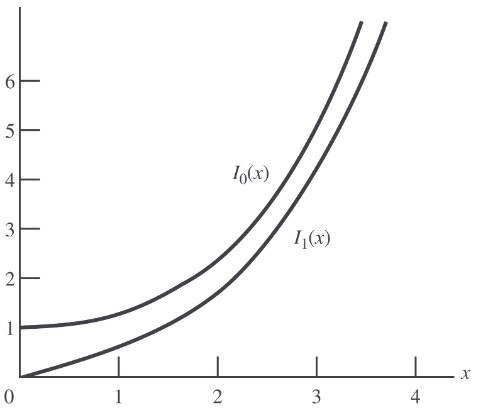
\includegraphics[height=5cm, keepaspectratio]{bessel1}
		\caption{}
		\label{fig:bessel1}
	\end{subfigure}
	\hfill
	\begin{subfigure}[t]{0.49\textwidth}
		\centering
		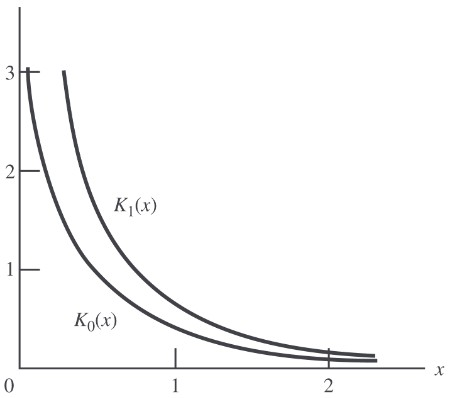
\includegraphics[height=5cm, keepaspectratio]{bessel2}
		\caption{}
		\label{fig:bessel2}
	\end{subfigure}
	\caption{Modified Bessel functions of the (a) first and (b) second kind and order $0$ and $1$. Reproduced from \cite{balanis1}.}
	\label{fig:bessel}
\end{figure}


%\subsubsection{Electromagnetic Boundary Conditions}\label{subsubsec:bessel}
%\subsection{Slow Wave Structures}\label{subsec:periodic}
%\subsection{The Impedance Concept}\label{subsec:impedanceConcept}
%\subsection{Transmission Line Theory}\label{subsec:transmission}
